\documentclass[12pt]{article}
	\usepackage{graphicx,amsmath,textcomp}
	\usepackage[round]{natbib}
	\usepackage[margin=3cm]{geometry}
	\linespread{1.3}
	\bibliographystyle{plainnat}
	\title{
		Group \#07 \\
		Bridge-00 \\
		18g, 1700N \\[1cm]
		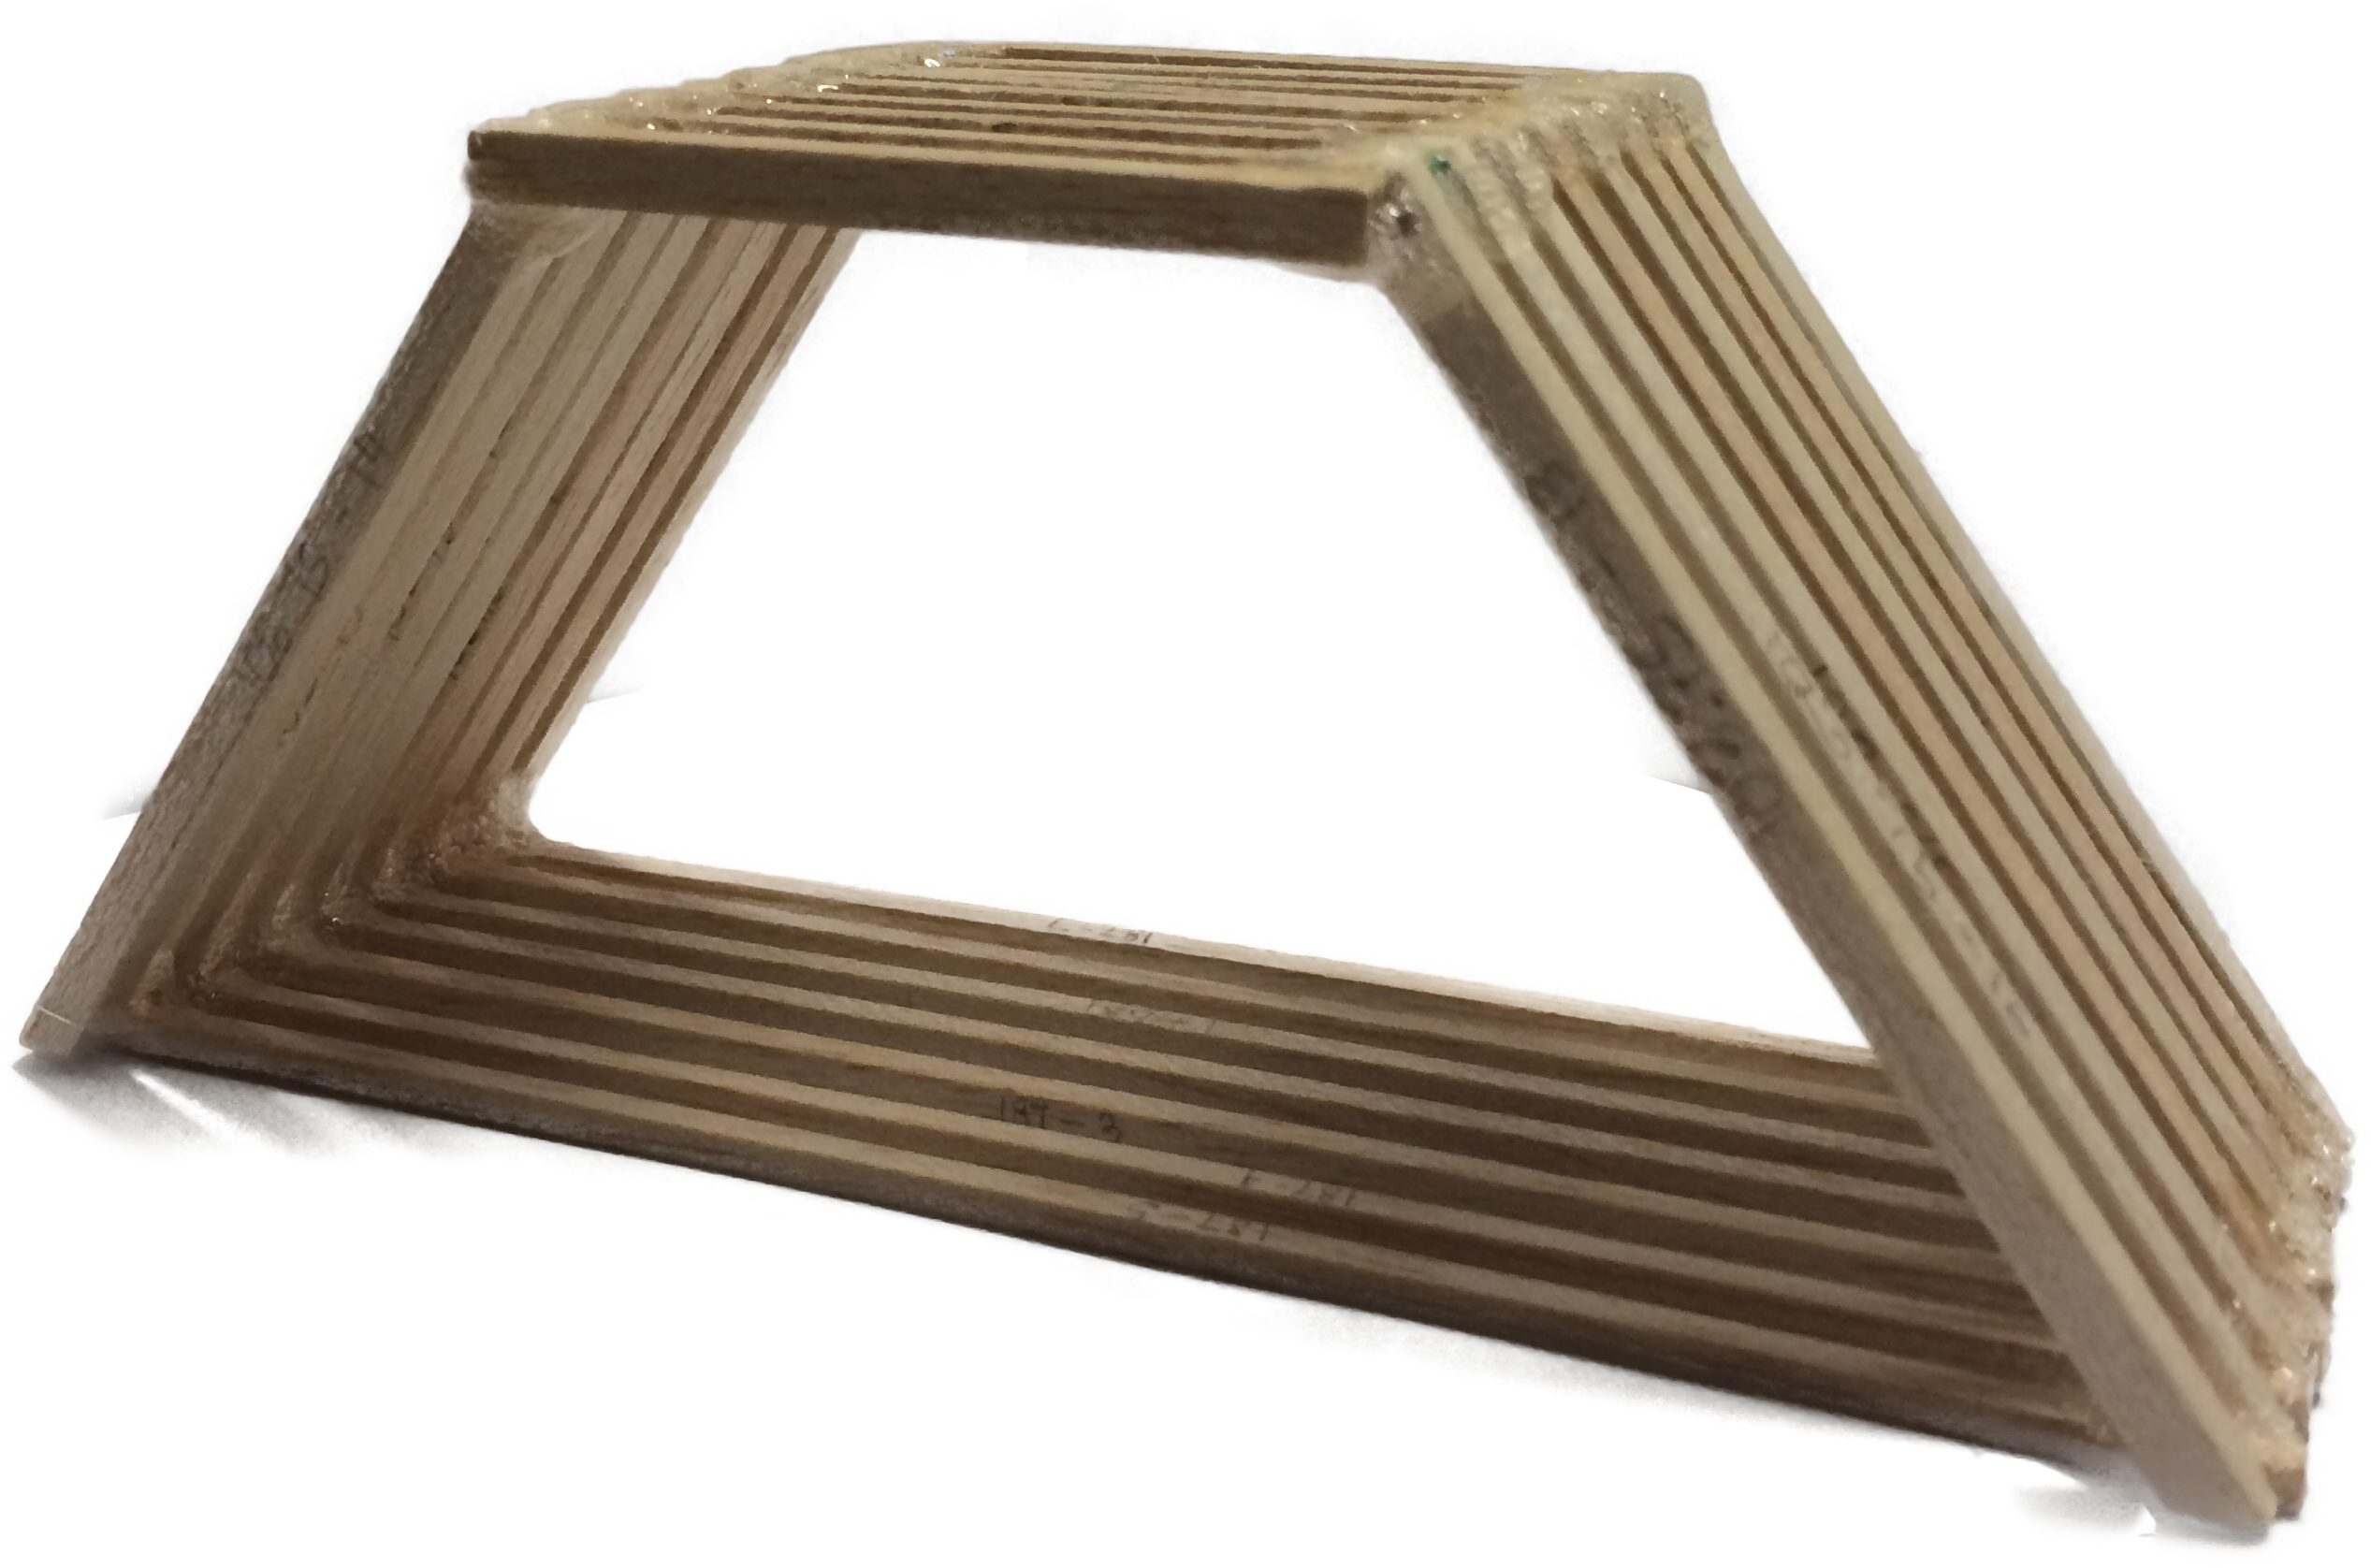
\includegraphics[width=0.7\textwidth]{photo}
	}
	\author{
		Alex Miles \\ u5568175 \\ 16.7\%
		\and Arlene Mendoza \\ u5589650 \\ 16.7\%
		\and Itsuki Nishida \\ u5578430 \\ 16.7\%
		\and Paul Apelt \\ u5568225 \\ 16.7\%
		\and Stephen Lonergan \\ u5349877 \\ 16.7\%
		\and Thomas Hale \\ u5568225 \\ 16.7\%
	}
\begin{document}
	\maketitle
	\thispagestyle{empty}
	\setcounter{page}{0}
	\section{Design}
		% design assumptions and methods
		\subsection{Assumptions}
		During the design process, the following assumptions have been made \citep[p.~264]{tbook}:
		\begin{enumerate}
			\item All loadings are applied at the joint,
			\item Weight of the members neglected,
			\item Joints are smooth (friction-less) pins,
			\item Each member has no more than two joints.
		\end{enumerate}

		\subsection{Considerations}
The task was set with a design criteria to span a gap of 180~mm and a width of 70~mm. The entire bridge also the bridge should weigh less than 18~g. The goal was to be able to hold the largest weight possible.

A very important design consideration was how many 2D truss panels should be used. The idea was by having more panels the design would be distributing the weight and if the layers span the 70~mm the design would be more efficient with its wood use. This is because we no longer need pieces holding the trusses together that don't add significantly to the strength of the design. This would be a better use of the wood as all of our wood would be focused on holding a load applied from above. 

Starting with a 70~mm wide layer of Warren trusses spanning 180~mm ran into a few problems. The largest limitation on the design was the materials allowed this meant the more triangles in the Warren truss the lower the truss had to be. This would create more smaller triangles which would increase the material. Several designs were looked at but it was found that spanning the gap required using a Warren truss didn't work due to the limited amount of material. However by removing all the triangles we had the outside of the truss which was in the shape of a trapezium. 

Another factor was also making sure that the force was applied onto the joints and not onto one member therefore the top of the bridge where the loading is applied should be less than 70~mm. The top of the bridge runs into the supports on both sides of the bridge and this transfers the load directly into the ground on either side of the trapezium. This takes advantage of the surface reactions. Because of this the more vertical the side pieces the better as they will distribute more of the force onto the support reactions rather than the other sections of the bridge. This is under the assumption that the sides don't break but if more force is downwards then some of the bracing stopping the bottom from slipping outwards wouldn't be needed and could instead could be moved to the sides.  

As these side pieces are taking the largest force it was decided to use the 5~mm pieces here. To stop the pieces from sliding out some of the 3~mm pieces on the bottom were used to hold the two ends of the design together and prevent slipping.The original design had half the pieces on the bottom as there were on the top. This bridge was tested rather imperfectly as the weight was skewed off centre and so broke earlier than expected. 

By moving two pieces of 5~mm to the sides of the top it was found that we could double the number of pieces along the bottom. Theoretically, the top and bottom of the truss take the same force and this is shown later in the calculations. By moving the 5~mm pieces to the top the top was 100~N stronger than the bottom and so the wood was being used efficiently as this gap is relatively small. The side supports while stronger would actually fail before the top does but after the bottom does and therefore the wood is being used very efficiently. The theoretical predictions for this later in the report shows that this is indeed the case.

One thing also considered but decided against was gusset joints, it was decided that gusset joints would not be used for for two reasons. One was that there were material constraints and that gusset jointing would be very similar to lamination where the joints would be situated, which wasn't allowed.

\subsection{Construction}
All the pieces were measured to the lengths in Table~\ref{list}, and they were then cut. Although the measuring was accurate, you lose some material whenever you cut. So to minimize loss of length, the pieces need to be cut in priority of one another. The 3~mm longest bottom pieces were cut first as these were extremely important to be at a full length. Total amount of material used is recorded in Table~\ref{materials}.
		\begin{table}[h!]
			\caption{List of member lengths.}
			\begin{center}
			\begin{tabular}{ | r | l | r | r | }
				\hline
				qty. & type & size & length \\ \hline
				7 & bottom & 3$\times$3~mm & 187~mm \\ \hline
				7 & top & 3$\times$3~mm & 70~mm \\ \hline
				2 & top & 5$\times$5~mm & 70~mm \\ \hline
				16 & sides & 5$\times$5~mm & 103.75~mm \\ \hline
			\end{tabular}
			\end{center}
			\label{list}
		\end{table}
		\begin{table}[h!]
			\caption{Materials used.}
			\begin{center}
			\begin{tabular}{ | r | r | r | }
				\hline
				size & given & used \\ \hline
				3$\times$3~mm & 1800~mm & 1799~mm \\ \hline
				5$\times$5~mm & 1800~mm & 1800~mm \\ \hline
			\end{tabular}
			\end{center}
			\label{materials}
		\end{table}

The leftover pieces were used to create the top of the bridge, these have the least priority as their length can be compromised if need be. Two 5 ~mm pieces are used on the top of the bridge. The 5~mm sides should be cut to the maximum length possible using the leftover material. Making them taller will distribute the more force into the support reactions. A small reduction in length would however not drastically reduce the maximum load. 

A template/scale diagram of the trapezium shape was then made to gain accuracy in the angles that needed to be attained (56\textdegree). Place the sides of the trapezium (5~mm) down with the top and bottom 3~mm pieces on top. Ignore the lone 5~mm top piece as this will be glued on last for ease of construction. Once enough glue (an amount when the two wood pieces are placed against each other that glue comes out from either side) was applied to the wood, the pieces were aligned to be at angles to each other and that the top and bottom pieces were in parallel. Weights were then placed to apply pressure to the joint. This would ensure the glue attains its maximum strength. The joints were then left to dry for each layer around 10 mins for another layer to be placed on top. The entire process was repeated until 8 layers were made.  The two 5~mm top pieces were then added to either side.The entire structure was then left to dry for 24+ hours.


		Final bridge design can be seen in Figures \ref{dim} and \ref{proj}.
		\begin{figure}[h!]
			\centering
			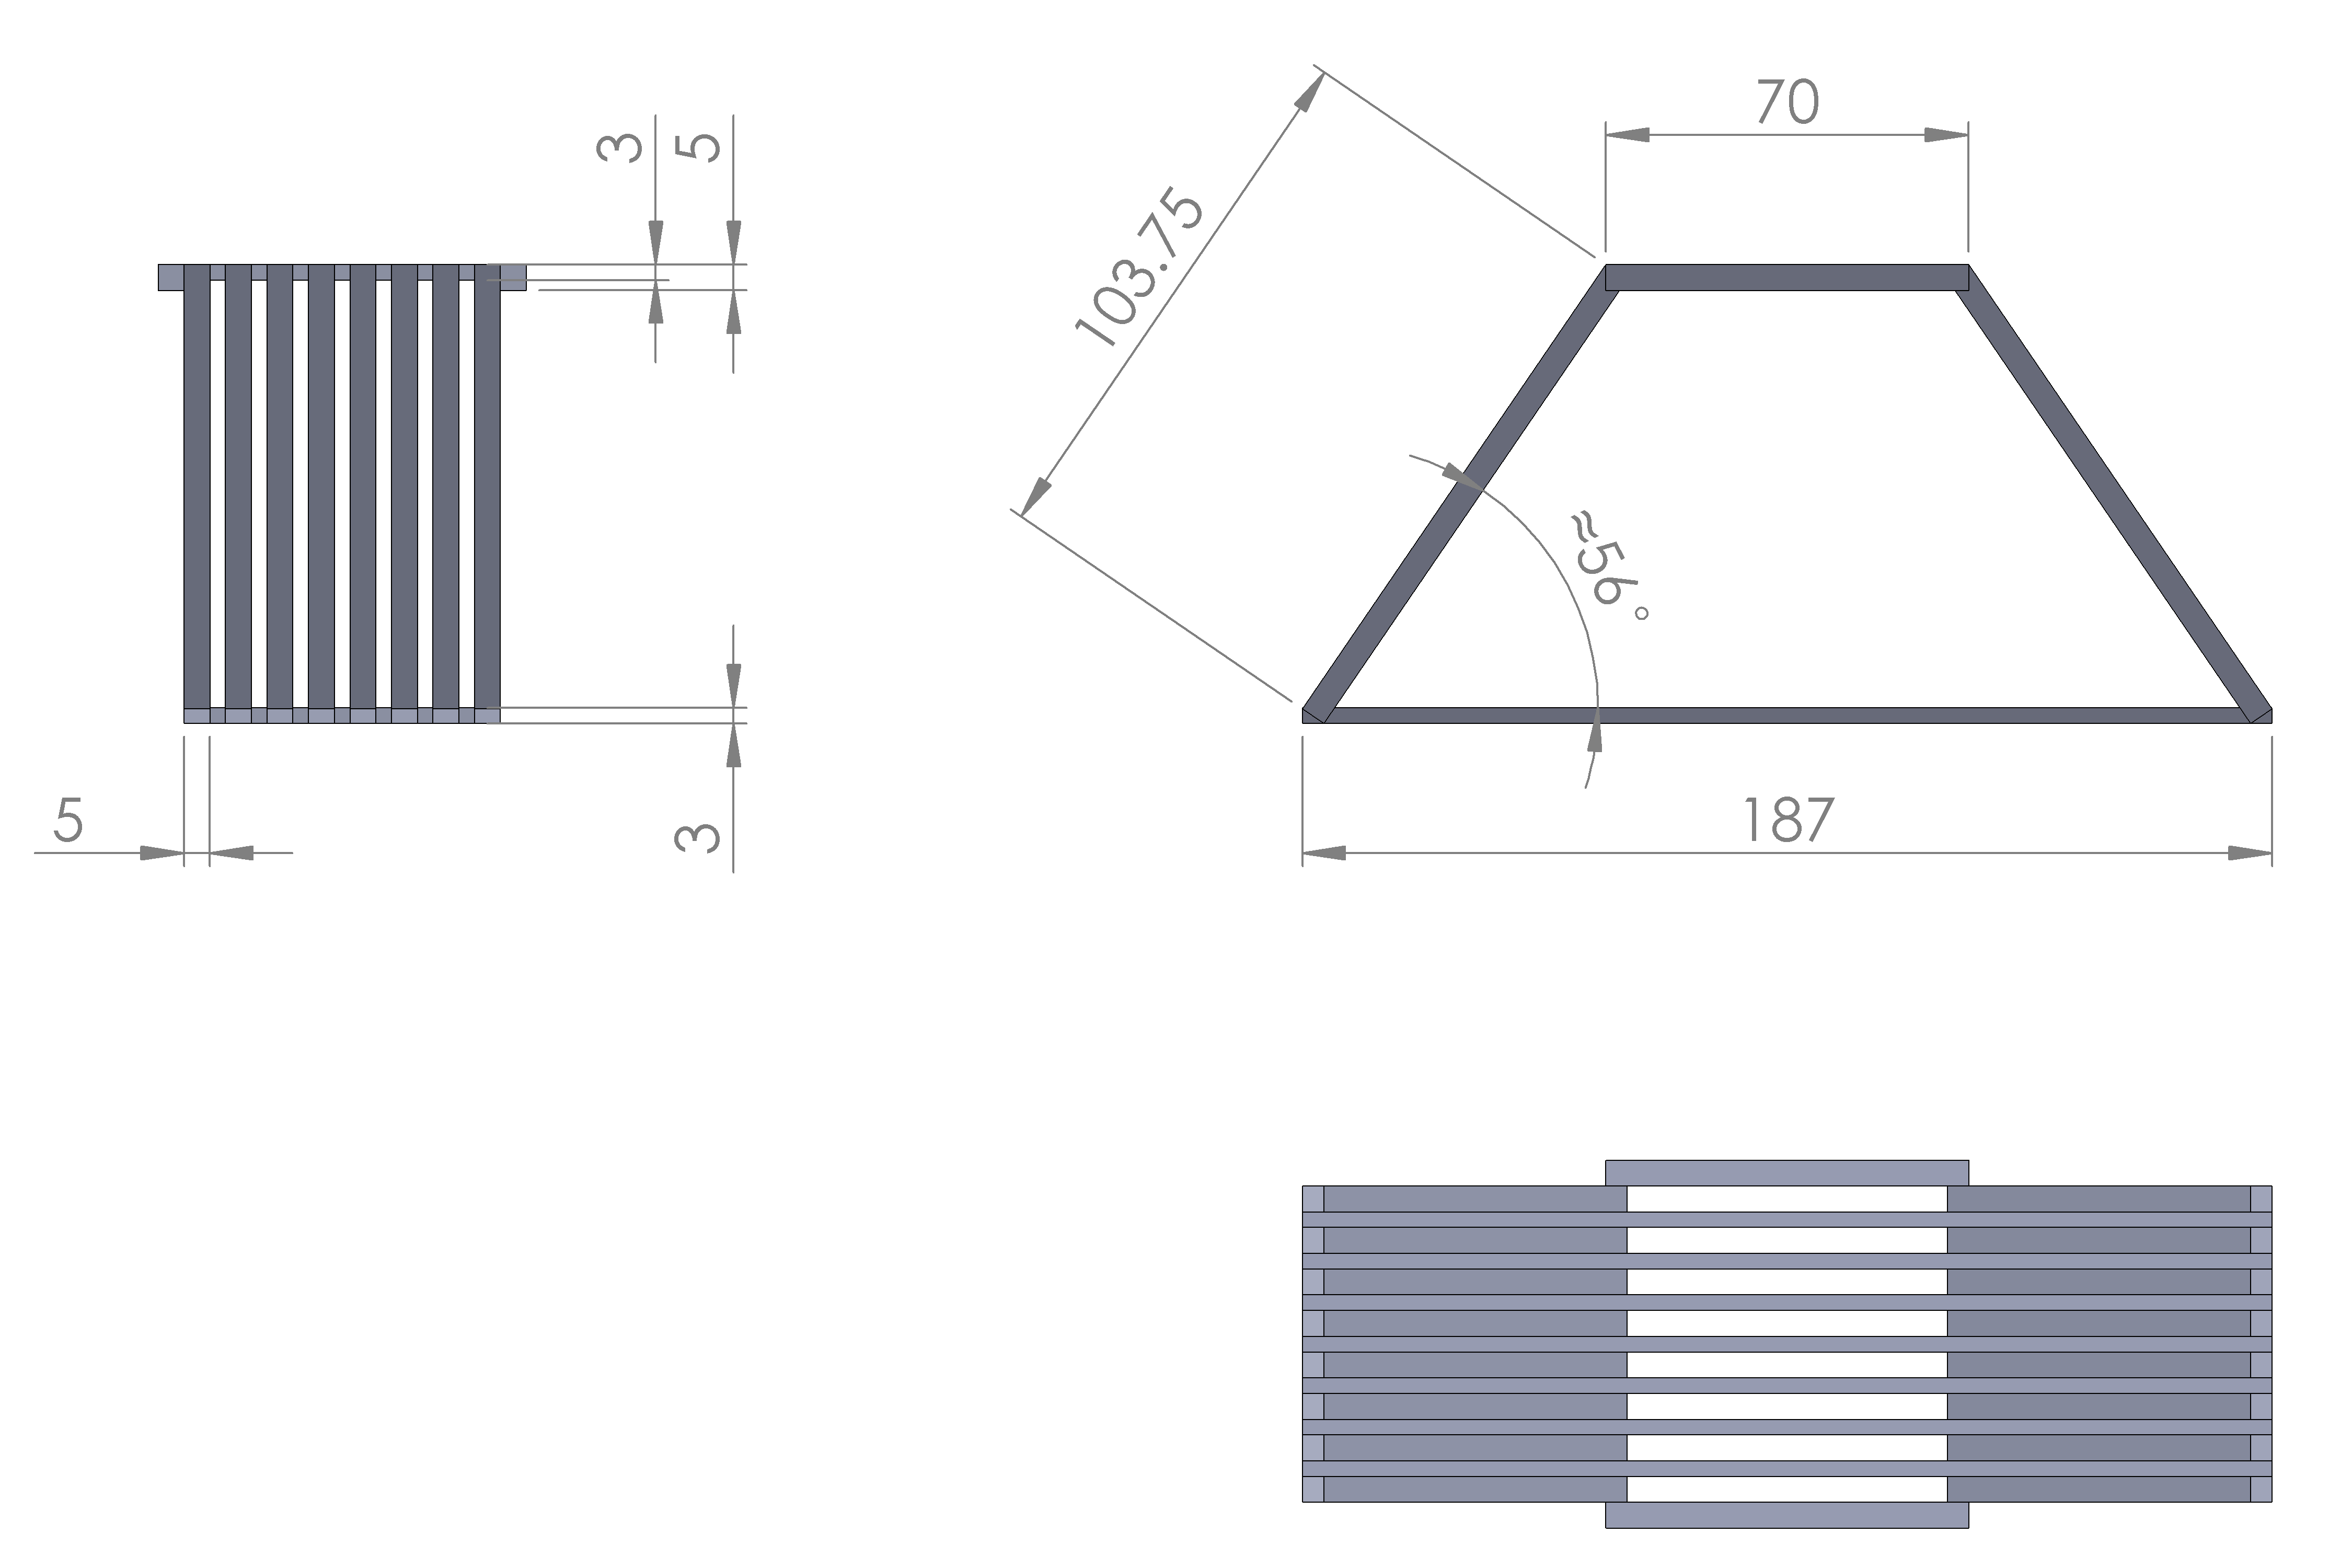
\includegraphics[width=\textwidth]{dim}
			\caption{Dimensioned drawing.}
			\label{dim}
		\end{figure}
		\begin{figure}[h!]
			\centering
			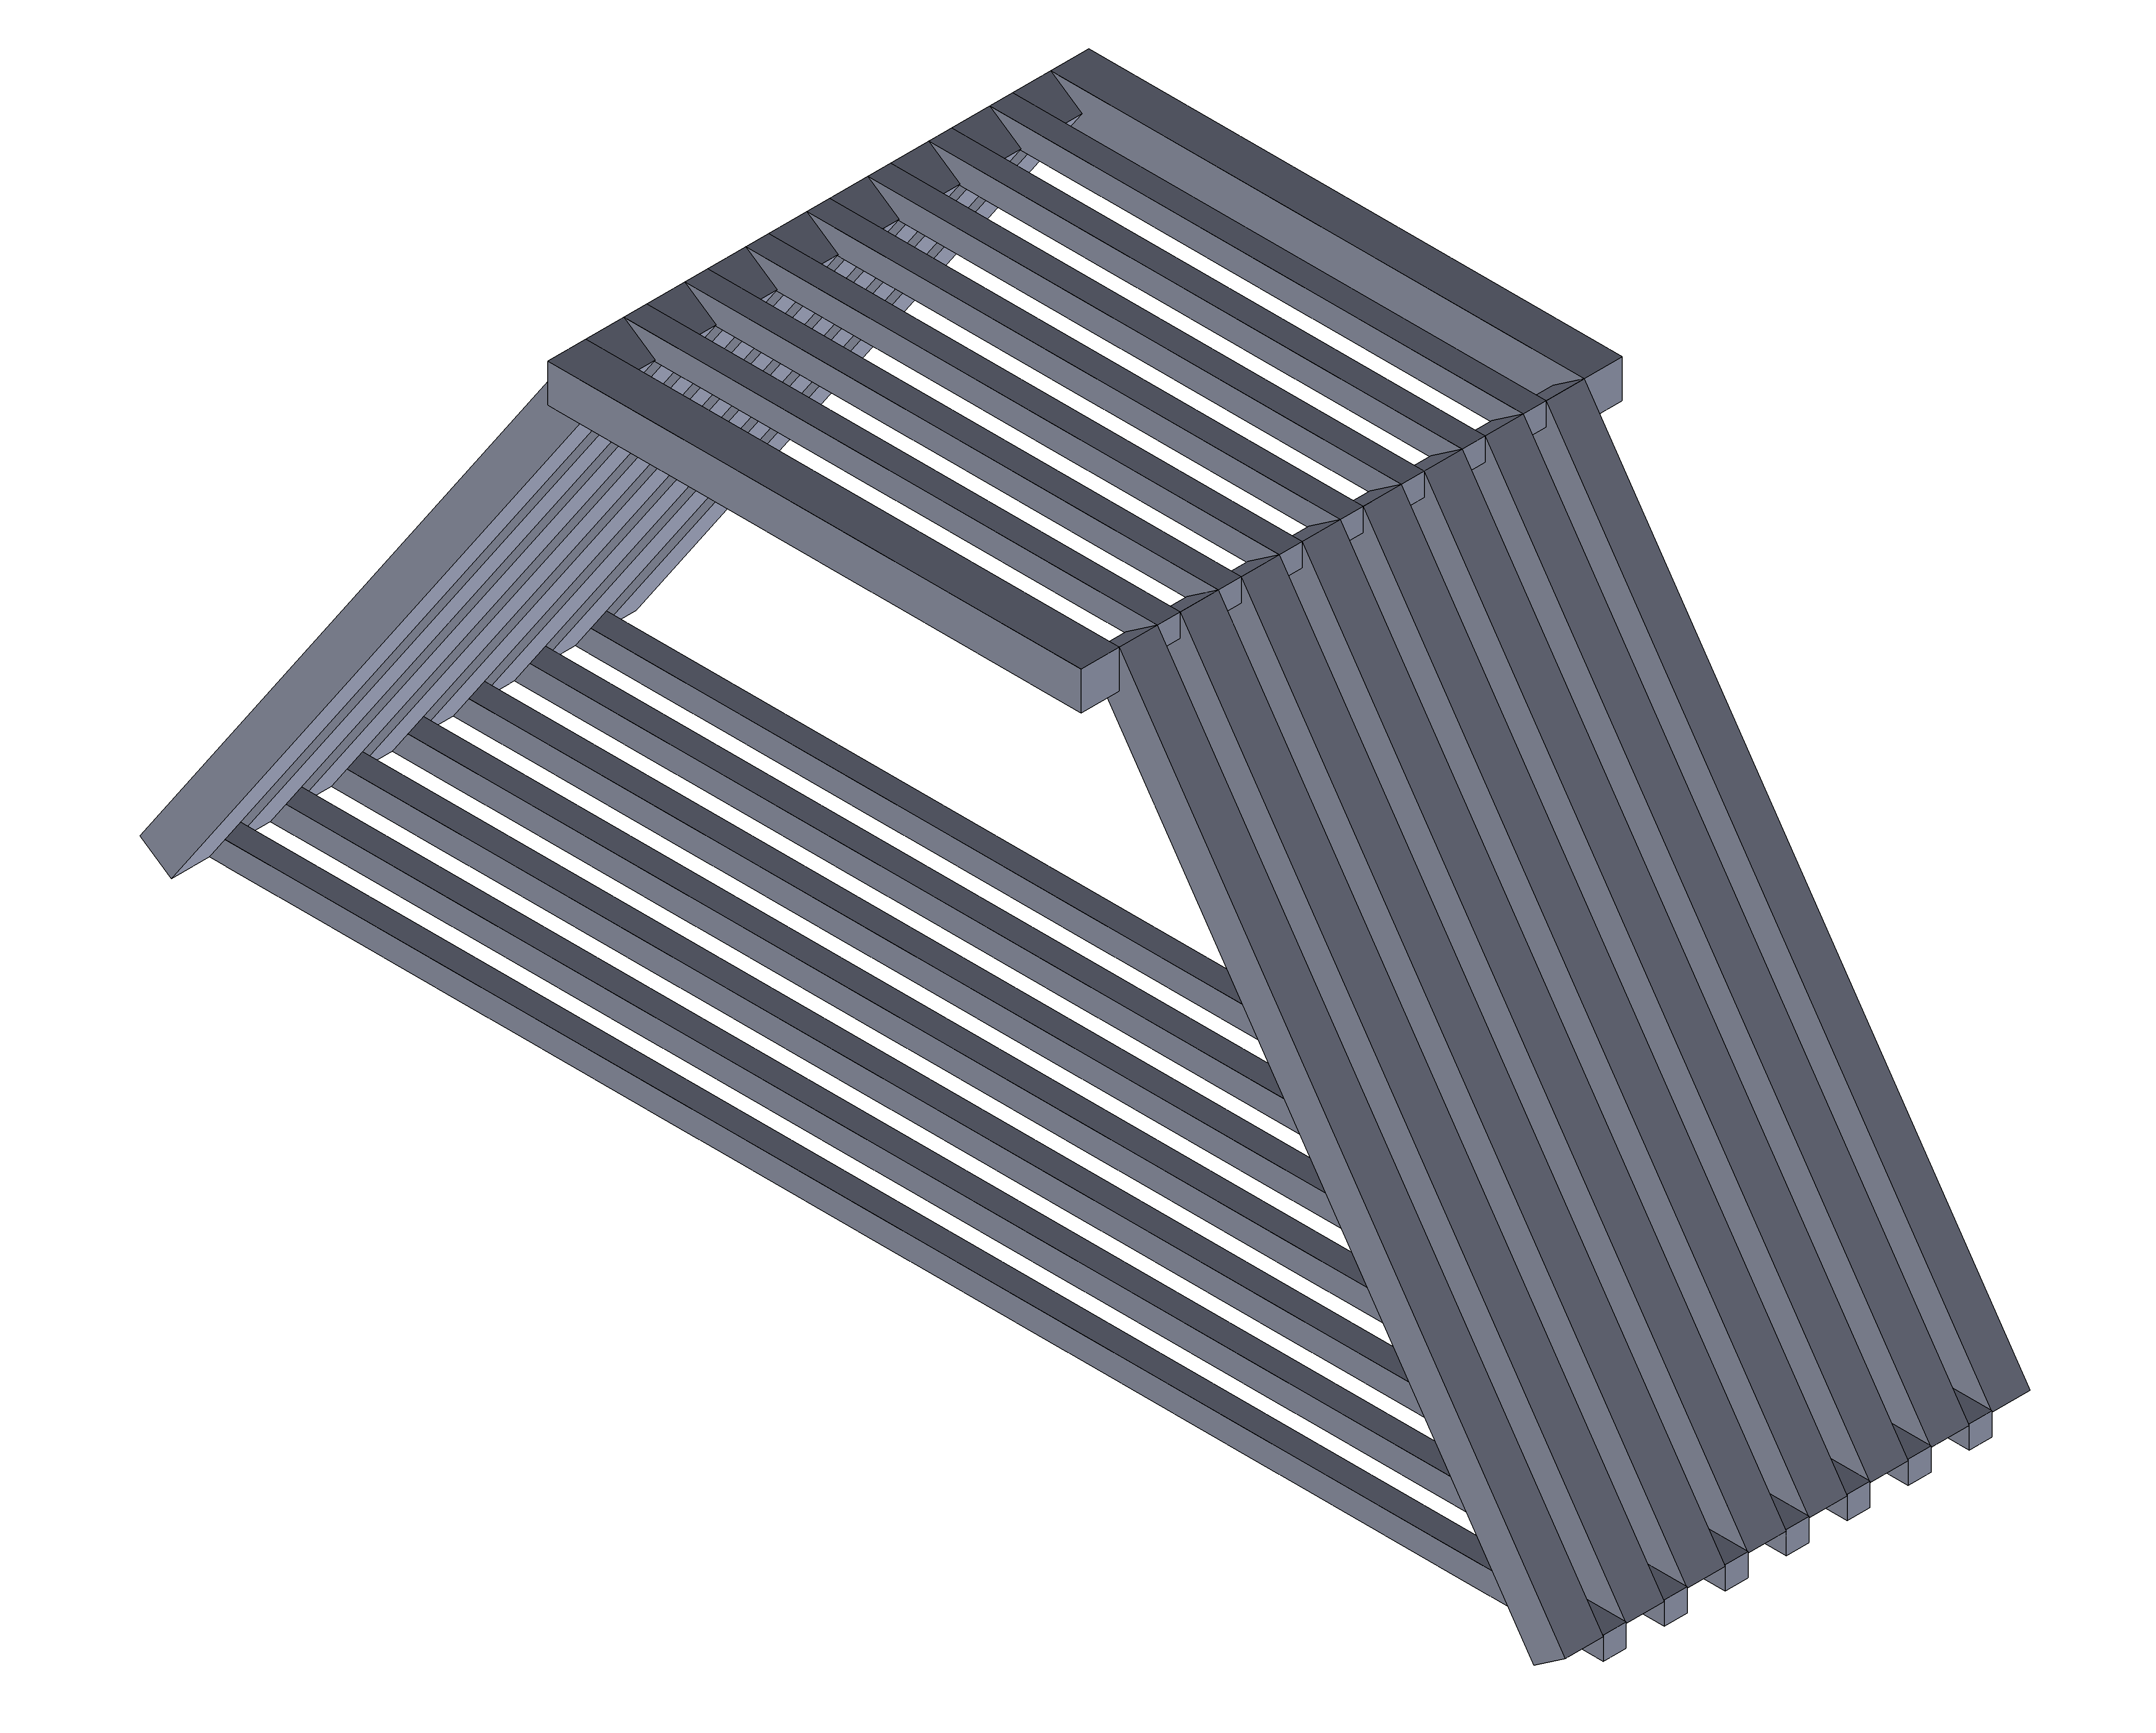
\includegraphics[width=0.5\textwidth]{proj}
			\caption{3D-Projection.}
			\label{proj}
		\end{figure}
		% dimensioned drawing
		
		% construction process 
		% materials Used
		% difficulties faced - measuring accurately, It ended up being 185~mm than 187~mm and the trapezium was also slightly lopsided by a 1~mm, angles are fucked!
		% weight issues - excess glue fail 
		% picture of the materials used
	\section{Analysis}
		Due to the unconventional design, to ease the calculations during the analysis, it was assumed that the load is equally distributed between eight trapezium-shaped trusses. Thus, a single trapezium truss was analyzed, and then extended to approximate the entire bridge. Internal forces, nodes and members are labelled as per Figure~\ref{trap}. As the truss is symmetrical, only two nodes needed to be analyzed.
		\begin{figure}[h!]
			\centering
			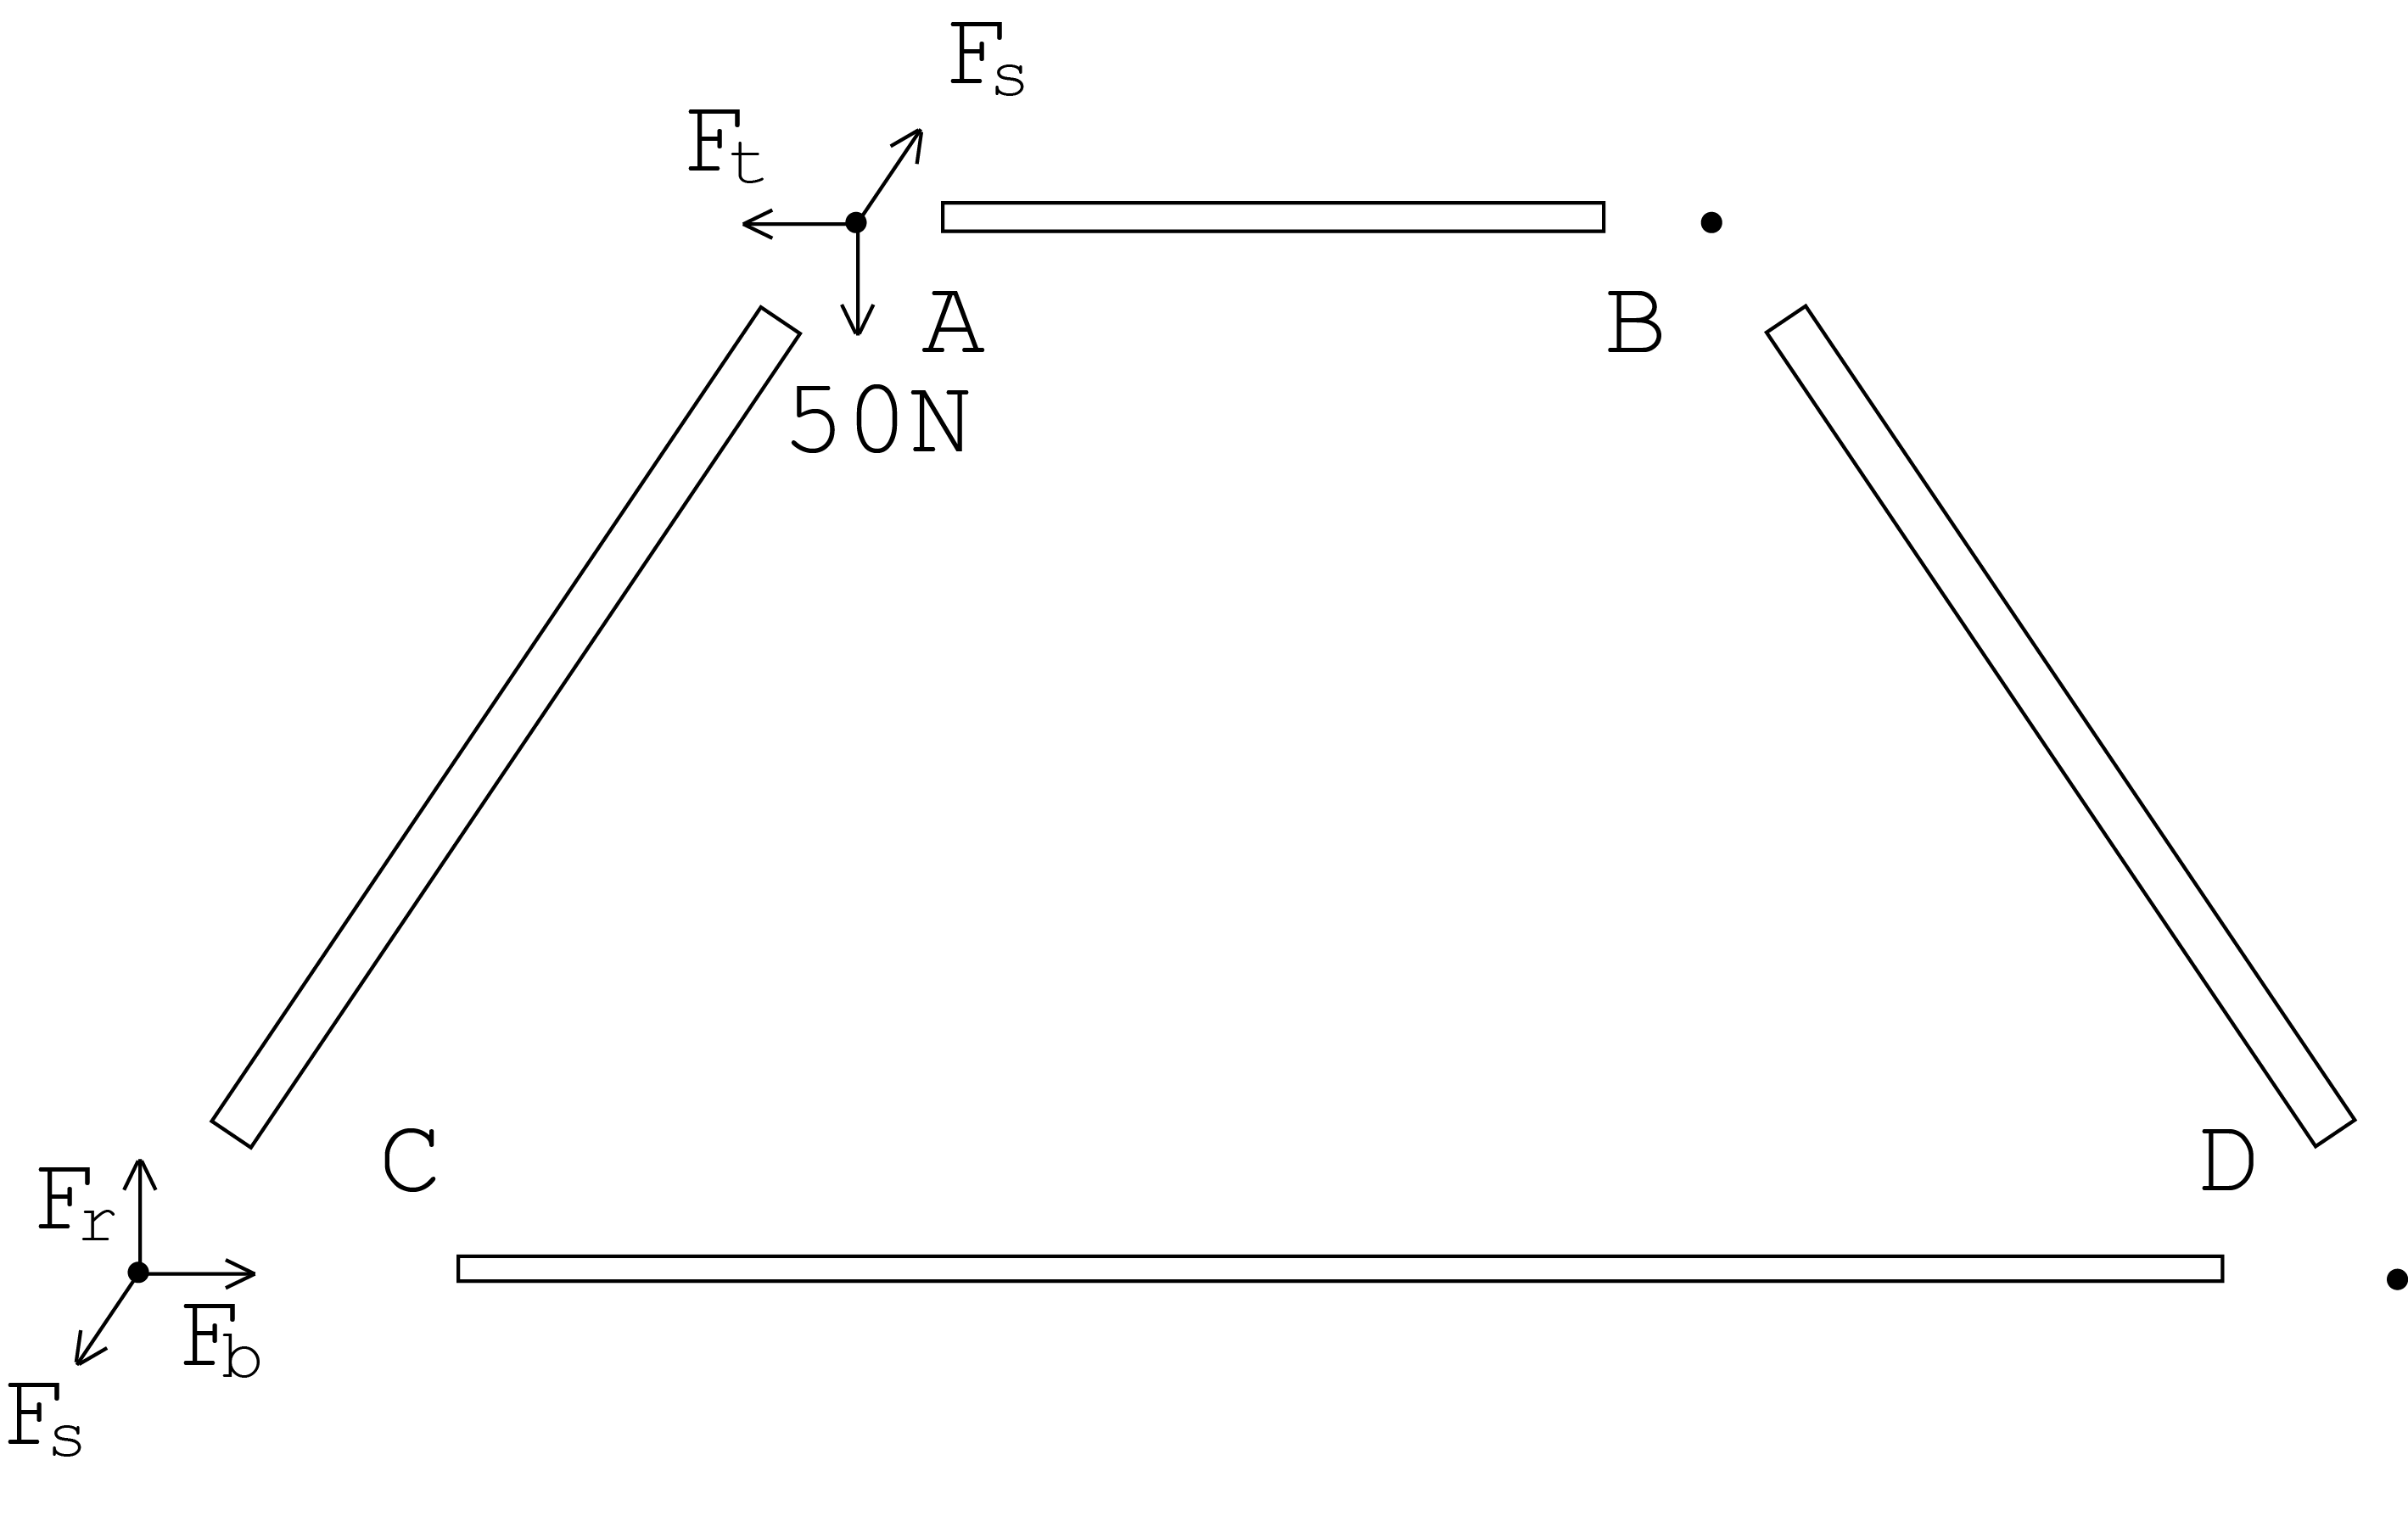
\includegraphics[width=0.5\textwidth]{trapanal}
			\caption{Trapezium truss.}
			\label{trap}
		\end{figure}
		For a load of 100N divided equally between nodes A and B, force equilibrium for nodes A and C are described in equation blocks \ref{eqn1} and \ref{eqn2} respectively.
		% insret calculations here
		\begin{subequations}
			\begin{align}
				F_s \sin 56&=50\mathrm{N}, \\
				F_s \cos 56&=F_t.
			\end{align} \label{eqn1}
		\end{subequations}
		\begin{subequations}
			\begin{align}
				F_s \sin 56&=F_r, \\ 
				F_s \cos 56&=F_b.
			\end{align} \label{eqn2}
		\end{subequations}

		The results of solving the above equations are presented in Table~\ref{loads}. Note that the internal force experienced by members is twice the given value, because it occurs at both ends.
		% table of member loads
		\begin{table}[h!]
			\caption{Member loads.}
			\begin{center}
			\begin{tabular}{ | r | l | }
				\hline
				70 3$\times$3 ~mm (top) & 33.7 N (c) \\ \hline
				103.75 5$\times$5 ~mm (side) & 60.3 N (c) \\ \hline
				187 3$\times$3 ~mm (bottom) & 33.7 N (t) \\ \hline
			\end{tabular}
			\end{center}
			\label{loads}
		\end{table}

		% assumptions
		% max load
		Maximum loads for each member were calculated using the values given in the Assignment sheet. Modulus of elasticity $E=3\mathrm{GN}/\mathrm{m}^2$, standard deviation $\sigma=+2.4/-2.1\mathrm{MN}/\mathrm{m}^2$. Tensile strength $\sigma_t=20\mathrm{GN}/\mathrm{m}^2$,  standard deviation $\sigma=+3.6/-3.4\mathrm{MN}/\mathrm{m}^2$. Compressive strength $\sigma_t=12\mathrm{GN}/\mathrm{m}^2$,  standard deviation $\sigma=+2.1/-2.8\mathrm{MN}/\mathrm{m}^2$. To calculate maximum load from strength values, equation \ref{eqs} was used. The results are presented in Table~\ref{maxloads}.
		\begin{equation}
			\sigma=\frac{P}{A}
			\label{eqs}
		\end{equation}
		\begin{table}[h!]
			\caption{Maximum member loads.}
			\begin{center}
			\begin{tabular}{ | r | l | l | }
				\hline
				& average & $-1\sigma$ \\ \hline
				3$\times$3 ~mm (c) & 108 N & 82.8 N \\ \hline
				3$\times$3 ~mm (t) & 180 N & 149.4 N \\ \hline
				5$\times$5 ~mm (c) & 300 N & 230 N \\ \hline
			\end{tabular}
			\end{center}
			\label{maxloads}
		\end{table}

		Buckling loads were calculated for members under compression (using equation~\ref{eqb}), and it found that the buckling loads of members under compression (see Table~\ref{buck}) did not exceed maximum load, therefore buckling was not critical.
		\begin{equation}
			P_b=\frac{\pi^2 E I}{(kL)^2}
			\label{eqb}
		\end{equation}
		\begin{table}[h!]
			\caption{Maximum buckling loads.}
			\begin{center}
			\begin{tabular}{ | r | l | l | }
				\hline
				& average & $-1\sigma$ \\ \hline
				3$\times$3 70 ~mm (c) & 163.1 N & 163.0 N \\ \hline
				5$\times$5 103.75 ~mm (c) & 573.1 N & 572.7 N \\ \hline
			\end{tabular}
			\end{center}
			\label{buck}
		\end{table}
		% reasons

		To predict the maximum load, the weakest section of the bridge had to be found. That was done by first su~mming up the maximum loads of all top, bottom and side members, (equation block~\ref{eqsa}), using values from Table~\ref{maxloads}, average column.
		\begin{subequations}
			\begin{align}
				P_{top}&=7\times108+2\times300
				&=1356\mathrm{N}\\
				P_{side}&=8\times300
				&=2400\mathrm{N}\\
				P_{bottom}&=7\times180
				&=1260\mathrm{N}
			\end{align}
			\label{eqsa}
		\end{subequations}

		Then the safety rations (defined in equation~\ref{eqr}) were calculated for each section (equation block~\ref{eqrl}), using values from Table~\ref{loads}.
		\begin{equation}
			R=\frac{P_{max}}{P}
			\label{eqr}
		\end{equation}
		\begin{subequations}
			\begin{align}
				R_{top}&=40.2\\
				R_{side}&=39.8\\
				R_{bottom}&=37.4
			\end{align}
			\label{eqrl}
		\end{subequations}

		The lowest safety ratio member will break first, thus bottom was determined to be the breaking point (snapping-type failure). The actual maximum load was determined in equation block~\ref{eqt}, where $P$ is the load used to calculate $R$. The same steps were carried out in equation block~\ref{eqs}, but the strength was assumed to be $1\sigma$ below average.
		\begin{subequations}
			\begin{align}
				F&=\frac{R P}{2} \\
				&=1869.4 \mathrm{N}
			\end{align}
			\label{eqt}
		\end{subequations}
		\begin{subequations}
			\begin{align}
				F&=\frac{R_{\sigma} P_{\sigma}}{2} \\
				&=1551.6 \mathrm{N}
			\end{align}
			\label{eqs}
		\end{subequations}

		The average of the two $1710.5\mathrm{N}$, was chosen as predicted maximum load.
	\section{Results}
The predicted strength of the bridge was 1716~N while the maximum force that it sustained during the test was 875~N. The most significant contributor to this imprecise prediction was that the bridge was too short to comfortably span the 18~cm gap. Furthermore, gluing techniques were not researched and as a result the joints were not as strong as they otherwise may have been.

Upon a load being applied to the top of the bridge, it became evident that the rear left corner did not have the length to fully span the gap. The rear 4 trapeziums immediately started to slip down into the gap below the block. This was ultimately the cause of the actual load being significantly below the predicted load. The four supported trapeziums at the front of the structure still held, and they performed as they were expected to. However, no member of the bridge actually failed. Other minor factors played a part, such as the bridge being slightly higher at the top in the rear and the overall strength of the glued joints. In an attempt to analyse why no member broke, the full sequence of events is laid out.

To prevent the rear left section of the bridge from instantly separating and falling down under the load, the joints needed to supply an upward force, equivalent to the downward force on the section. This resulted in a shear force on the 5th joint on the upper left hand side, a shear force on the 4th joint on the lower left hand side, and moments about the corresponding joints on the left hand side. Joints are labelled in figure~\ref{AnalysisLabelled}.


		 
		   \begin{figure}[h!]
                 	\centering
			\begin{minipage}[b]{0.45\linewidth}
			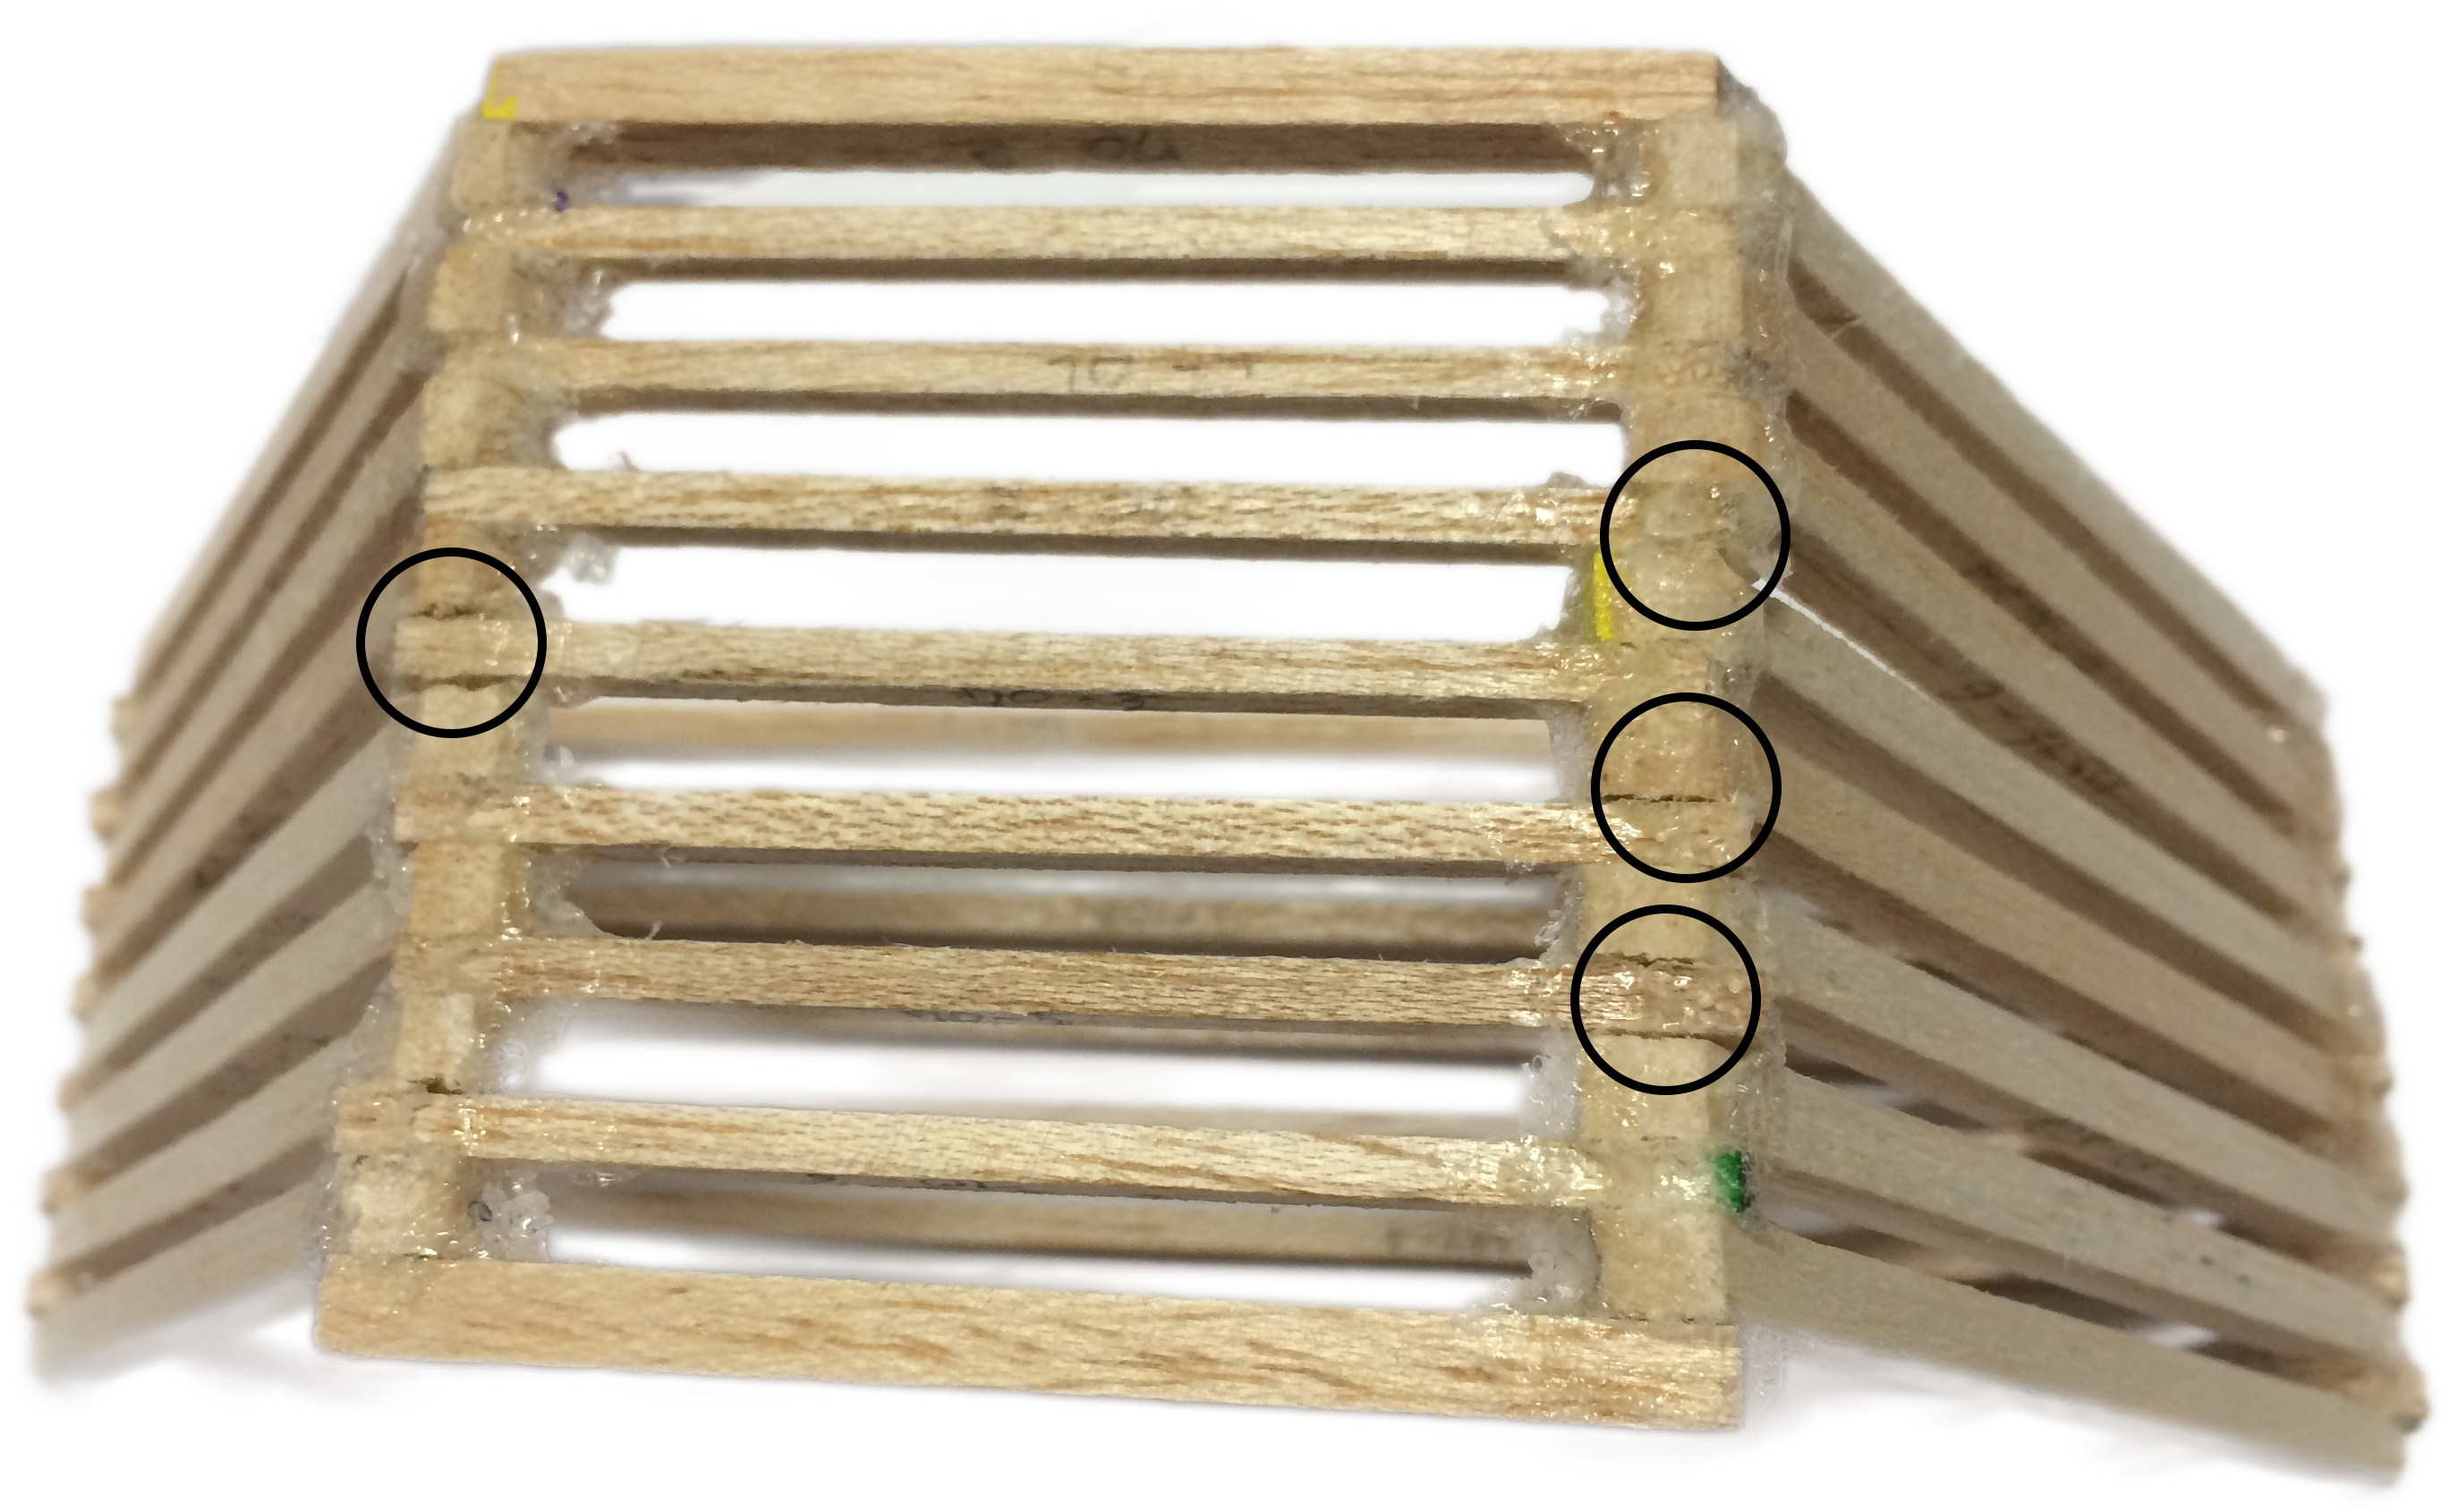
\includegraphics[width=1.1\textwidth]{failtop}
			\caption{Failure points on the top of the bridge}
			\label{failtop}
		\end{minipage}
		\quad
	\begin{minipage}[b]{0.45\linewidth}
			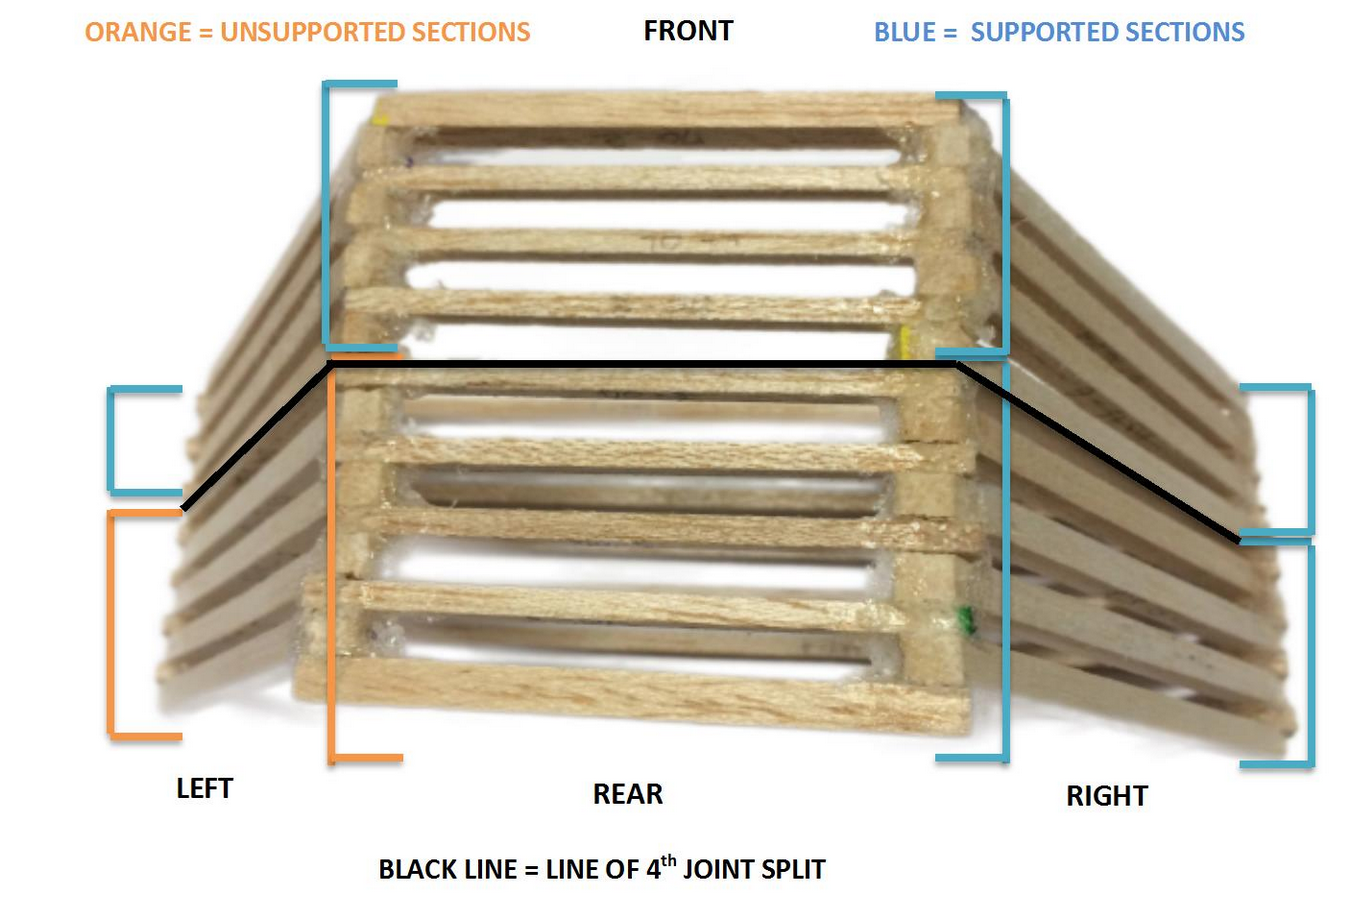
\includegraphics[width=1.4\textwidth]{AnalysisLabelled}
			\caption{Labelled Sections}
			\label{AnalysisLabelled}
		\end{minipage}
		\end{figure}
             
The balsa glue itself has a reasonably high degree of elasticity under both torsional and shear forces, with the ability to be displaced several millimetres prior to failure. 

The moment about the two right-side joints was also counteracted by the glue. As was shown in our tests (see appendix), the maximum torsional force (light fibre-tear failure) is roughly one third the maximum shear force (cohesive failure). Double gluing may possibly have spread this torsional force through a larger volume of cement, allowing it to withstand a larger force prior to failure. 

The joints on the left hand side however, were more susceptible than the right hand side. The joints on the left had separated by about 2~mm prior to failure. Due to the much higher shear strength this was unexpected, however, the balsa glue having a high elasticity was what enabled this. The span of the bridge meant that the right joints had only rotated between 0\textdegree and 2\textdegree approximately, while during testing they were able to maintain rotation of up to 45\textdegree prior to failure, which was when the max force was reached. There was also a small shear force on each joint on the right, but the glue was able to absorb this at this time, as it was significantly less than the shear on the left joints.

After the glue had reached a critical length on the left hand joints, it sheared, leaving little to no support on this side for the first 4 trapeziums, which was shown by them sinking significantly into the gap.

The only support the section had at this time on was from the two joints on the right hand side, which were now experiencing a large moment, combined with a shear force. 

Through testing, the maximum moment for a heavily glued joint was about $28$ -- $30\mathrm{Nm/cm^2}$ of glue. The glue was estimated to have been applied to about $1\mathrm{cm^2}$, the maximum moment in a joint would be about $28$ -- $30\mathrm{Nm}$ and the maximum shear about $65$ -- $80\mathrm{N}$. 

The trapeziums appear to flatten out as the top moves to the left, so the load is still distributed at this point, as seen in figure ~\ref{load top} However, due to the slant of the bridge, the rear trapeziums had a much higher load than the front ones, causing a large shear force to build up in the upper and lower right joints, going from the rear to the supported section as they failed one by one. This suggests that the joints did not fail due to the moment. ($30 / 0.035 = 8570\mathrm{N}$) which would be the required resultant distributed force half way along the top of the bridge. 

 			\begin{figure}[h!]
				\centering
				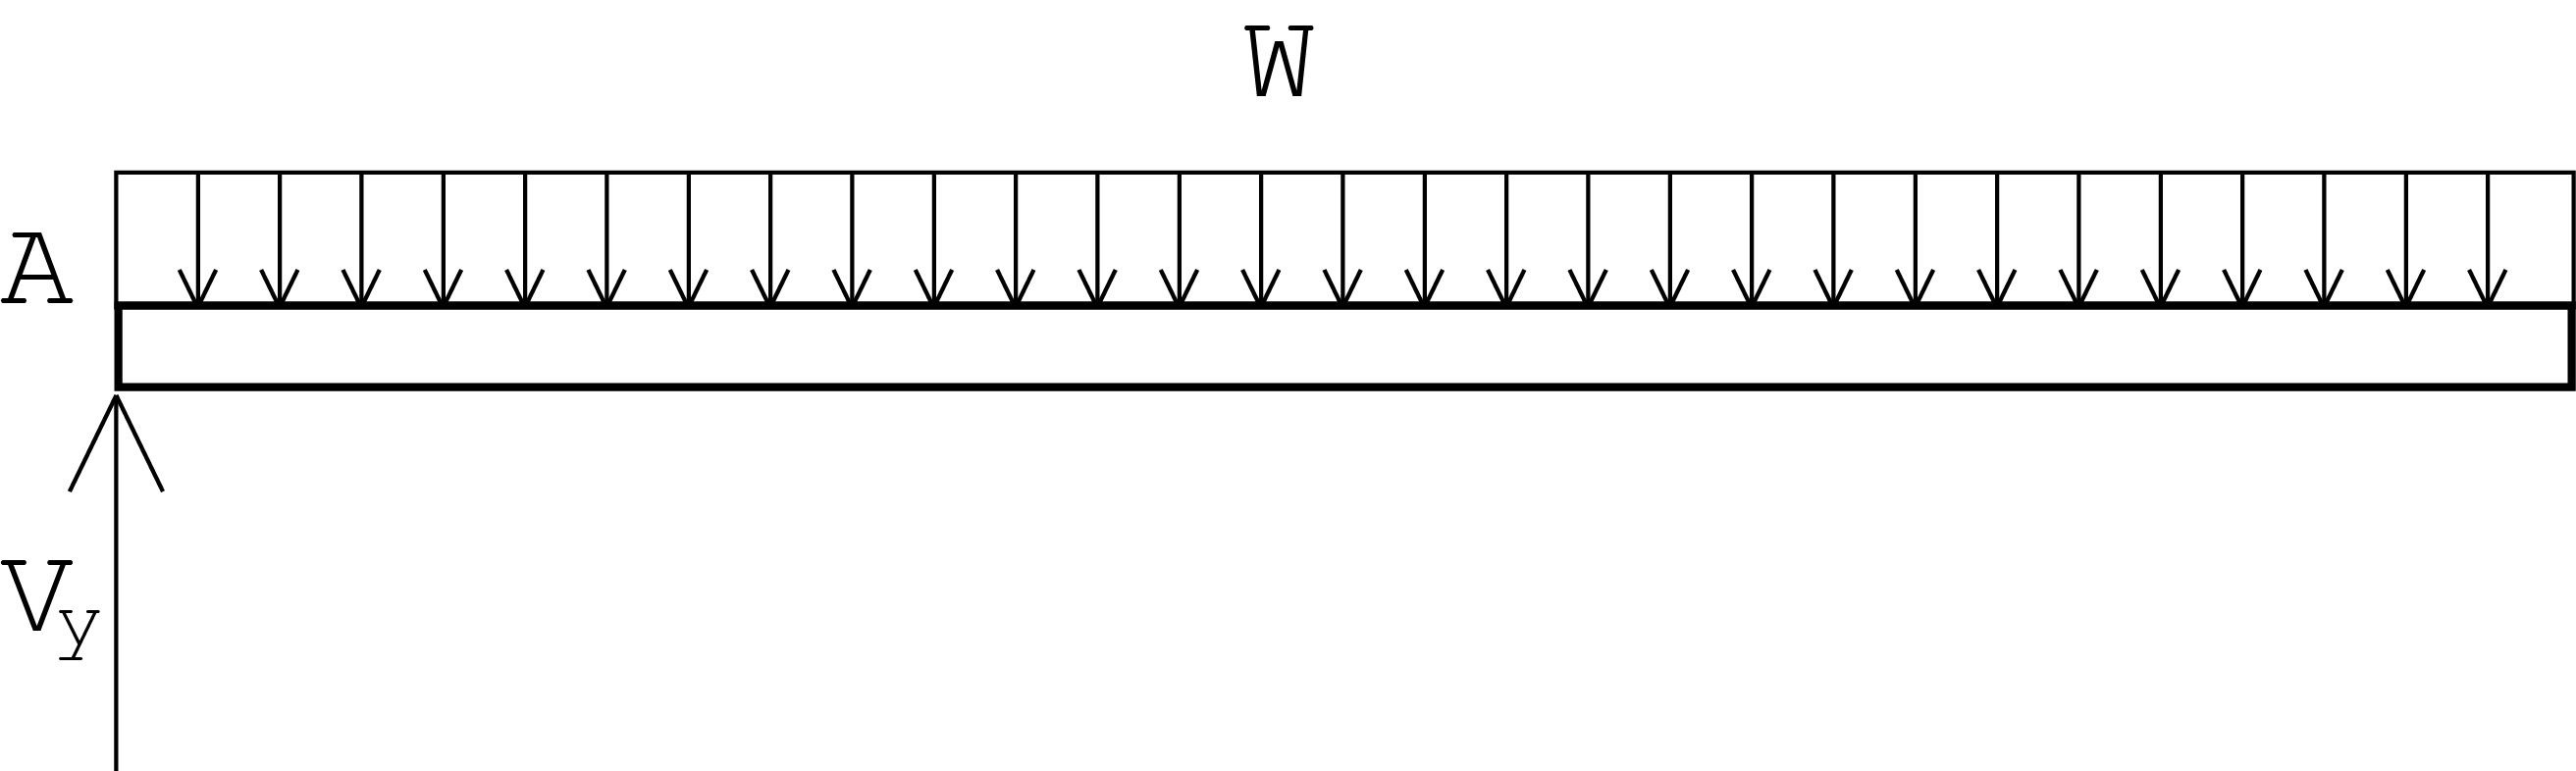
\includegraphics[width=0.35\textwidth]{loadtop}
				\caption{Half of the top joint row under load}
				\label{loadtop}
				\end{figure}

The force exerted on each trapezium would need to exceed a minimum of 130~N, to shear the two joints. It appears that the top joint would fail, allowing the trapezium to shift in shape farther to the left. This converted the shear in the lower joint to a torsional force, which was absorbed by the glue. 

The joints of concern all failed within this range, the distributed load gradually evened out as the top flattened, but the load was estimated to be under 200~N by the time the last joint failed. 
Consequently, the rear 4 trapeziums were supporting almost none of the load. This was illustrated when the loading was removed and the bridge does not return to its original position.

This left the remaining force to be supported by the functioning 4 trapeziums, which gradually took the load as was predicted, with the bottom spreading slightly as the tension in the lower members was increased. Having only one half of the bridge remaining, the maximum load dropped to half the predicted value ($1716 / 2 = 850\mathrm{N}$). If the bridge had not been too short a failure should have occurred around this region. It was predicted that a lower member would break, however, this did not occur due to joint failures. Therefore the the final four trapeziums crossed the max threshold for the elasticity of the glue in the joints, and began to slip, due to the large volume of glue used, it has strong elastic deformation. This value was roughly equivalent to the breaking force of the lower members (10 upper moments and 7 lower shear forces/moments; this is the number of $\mathrm{cm^2}$ in joints, $3.5 \mathrm{cm^2}$ on each side) This gives a value of ($875\cos 56 = 489\mathrm{N}$). The value for failure of 7 shear joints is $65$ -- $80\mathrm{N}$ each, giving a value between $455$ and $560\mathrm{N}$. Due to the small torsional force in the joints, on top of the shear, the value is in the lower range of the estimate. A deviation in the actual surface area of the glue creates some room for error in this. Though, this range matches the tested value.  At this point, a joint slipped, registering a decreased load, stopping the machine and consequently preventing a structural failure.
\clearpage
\bibliography{bib}
\clearpage
\section*{Appendix}
%glue stuff here
After the bridge had undergone the final test and did not perform as well as we had hoped, we decided to test further the the joint strength at varying amounts of glue. 40 tests using 8 cm 5mm balsa wood pieces were glued together like seen in figure 7.
                \begin{figure}[h!]
			\centering
			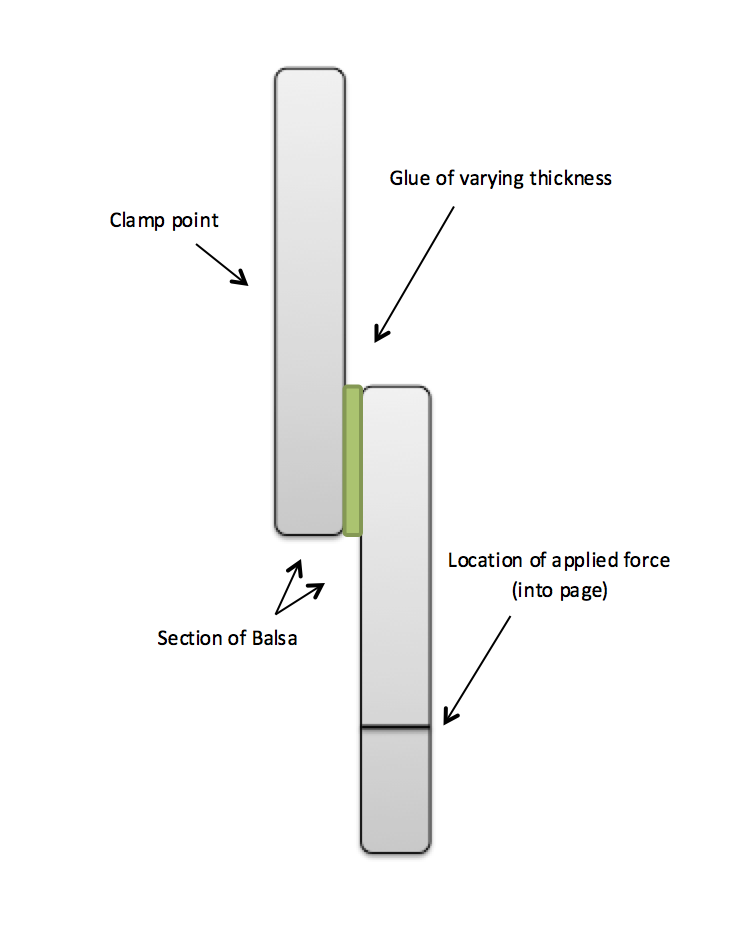
\includegraphics[width=0.3\textwidth]{Jointtest}
			\caption{Joint Tests}
			\label{Joint Testing}
		\end{figure}

There were 4 groups that we decided on testing; a very small amount (A), a thin layer (B), a sufficient amount so that glue spills out from the sides of the joint (C) and a very thick layer of glue, making a visible layer between the joints, - with overflow -  similar to our bridge (D).
We wanted to test the weight the joint could hold before the wood itself or the glue joint broke.

To test, the joints were clamped at to the surface of a table with half the joint hanging off, and the other half on. 1N weights were progressively hung off  the unsupported member, to simulate a gradually increasing force. The weight was applied at a constant distance from the edge of the joint so the moment was consistent for our 40 tests.
The data collected can be seen in figure 8 and the graph in figure 9, where group 1,2,3 and 4 correspond to A, B, C and D accordingly.
		
                \begin{figure}[ht]
                 	\centering
			\begin{minipage}[b]{0.45\linewidth}
			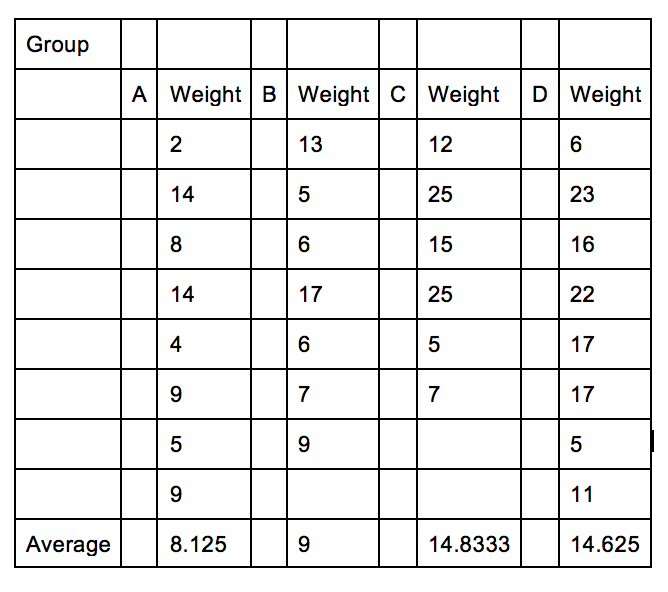
\includegraphics[width=1\textwidth]{GlueResults}
			\caption{Glue Joint Results}
			\label{fig:minipage1}
		\end{minipage}
		\quad
	\begin{minipage}[b]{0.45\linewidth}
			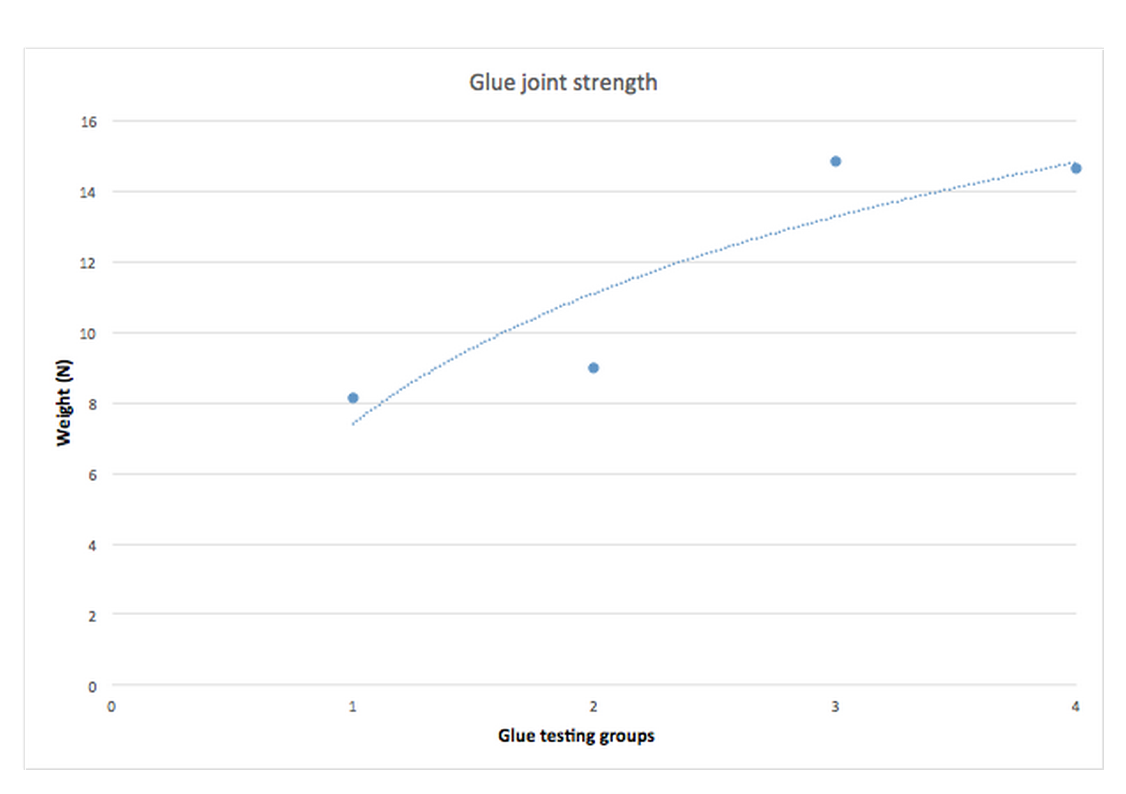
\includegraphics[width=1.2\textwidth]{GlueGraphlegit}
			\caption{Joint strength graph}
			\label{fig:minipage2}
		\end{minipage}
		\end{figure}
                
              
We also carried out a few tests on the shear force of the joints, however, due to the impracticality of the measuring procedure, only a small number of tests were able to be conducted. The average of these tests was measured to be 32N.
                 
                 \begin{figure}[h!]
                          \centering
                          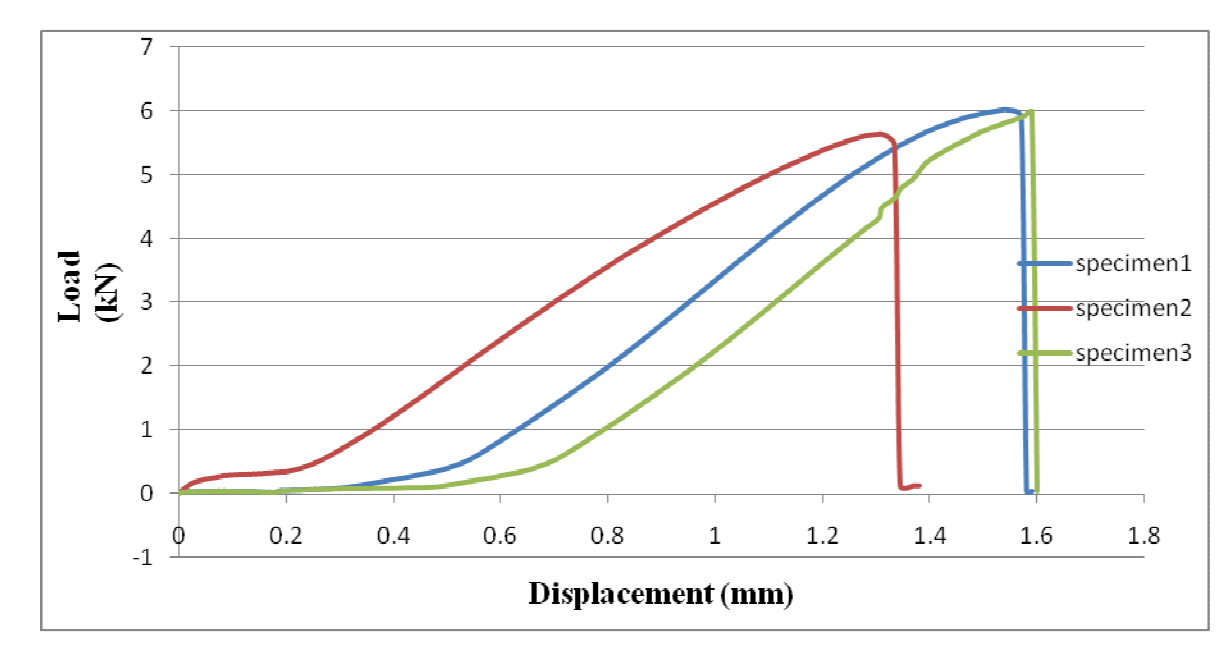
\includegraphics[width=0.4\textwidth]{Articlegraph}
                          \caption{(Mohamed Bak,2012)}
                          \label{GraphGlue}
                 \end{figure}
Our hypothesis before the testing was that the strength of the glue will increase up until a point at which the strength plateaus then will drastically drop. We also predicted that the joint would display a reasonably high degree of elasticity, prior to the joint failing. 

The testing that was implemented does show these results but not enough tests were carried out to view the dramatic drop in strength. Around ~1000 tests would have to be carried out in order to view this. 
Fortunately, the elasticity was demonstrated from the tests we did. The more glue the joint had, the higher the angle it could rotate to prior to failing. Some of these joints were able to reach roughly 45\textdegree rotation from their starting position, prior to failing. This suggests that increasing the volume of glue further would have allowed a higher degree of rotation, as the glue absorbed some of the force. The force absorbed by the glue would have an impact on the balsa not failing, however, cohesive failure would still occur at a high enough force.

These results do prove that maybe glue was an issue with the joints as a lot of glue was used to reinforce the joints.
The graph in figure 10 shows the results that we were aiming to achieve.
\end{document}
